\documentclass[a4paper]{article}

\usepackage[a4paper, top=8mm, bottom=8mm, left=8mm, right=8mm]{geometry}

\usepackage{polyglossia}
\setdefaultlanguage[babelshorthands=true]{russian}
\setotherlanguage{english}

\usepackage{fontspec}
\setmainfont{FreeSerif}
\newfontfamily{\russianfonttt}[Scale=0.7]{DejaVuSansMono}

\usepackage[tiny, compact]{titlesec}

\usepackage{titling}
\setlength{\droptitle}{-1cm}
\pretitle{\begin{center}\begin{bfseries}\Large}
\posttitle{\par\end{bfseries}\end{center}}
\preauthor{\begin{center}\normalsize}
\postauthor{\par\end{center}\vspace{-1.8cm}}

\usepackage{hyperref}
\usepackage{bookmark}
\usepackage{csquotes}
\usepackage{enumitem}
\usepackage{amsmath}
\usepackage{graphicx}

\title{Реализация свёртки изображений на Python}

\author{Бывалкина Мария Дмитриевна}

\date{}

\begin{document}

\maketitle

\begin{flushright}
    Группа: \emph{\enquote{25.Б43-мм}}

    Кафедра: \emph{системного программирования}

    Научный руководитель: \emph{Пономарев Николай Алексеевич}

    Номер семестра практики: \emph{2}
\end{flushright}

\section{Введение}

Обработка изображений является одной из важных задач современного программного обеспечения. Она используется в системах компьютерного зрения, медицинской диагностике, графических редакторах и многих других областях.

Свёртка является из базовых операций обработки изображений. Данная операция позволяет изменять изображение при помощи специальной матрицы коэффициентов, называемой ядром свёртки. В зависимости от выбранного ядра можно выполнять размытие изображения, повышение резкости, выделение контуров и другие преобразования.

Математически двумерная свёртка изображения $I$ с ядром $K$ определяется следующим выражением:
\[
(I * K)(x,y)=
\sum_{i=-r}^{r}
\sum_{j=-r}^{r}
I(x+i,y+j)\cdot K(i,j),
\]
где $r$ --- половина размера ядра.

Целью данной работы является разработка собственной реализации свёртки изображений на языке Python, проверка её корректности и сравнение производительности с существующими библиотечными решениями.

\section{Постановка задачи}

Цель практики заключается в реализации алгоритма двумерной свёртки изображений и проведении экспериментального исследования его производительности.

Для достижения поставленной цели необходимо решить следующие задачи:
\begin{itemize}
    \item реализовать операцию свёртки для полутоновых и цветных изображений;
    \item реализовать набор свёрточных ядер;
    \item обеспечить корректную обработку границ изображения;
    \item разработать тесты для проверки правильности работы алгоритма;
    \item провести сравнение производительности собственной реализации с библиотеками OpenCV и Pillow;
    \item визуализировать результаты измерений.
\end{itemize}

\section{Описание реализации}

Проект реализован на языке Python и построен на основе объектно-ориентированного подхода. Основная функциональность свёртки изображений инкапсулирована в классе ImageConvolution, который содержит методы для выполнения операции свёртки и различных режимов паддинга.

Для хранения и обработки изображений используются библиотеки Pillow и NumPy. Представление изображения в виде массива NumPy позволяет эффективно выполнять математические операции над пикселями.

\subsection{Поддержка цветовых режимов}

Программа поддерживает работу как с изображениями в оттенках серого, так и с RGB-изображениями.
Для полутоновых изображений свёртка применяется непосредственно к двумерному массиву яркостей.
Для цветных изображений обработка выполняется отдельно для каждого цветового канала (красного, зелёного и синего), после чего результаты объединяются в итоговое изображение.

\subsection{Обработка границ изображения}

При вычислении свёртки для пикселей, расположенных возле границ изображения, часть элементов ядра выходит за пределы массива. Для корректной обработки таких ситуаций реализован механизм дополнения изображения по краям.

В проекте используются следующие режимы дополнения:
\begin{itemize}
    \item \textbf{zero} --- заполнение отсутствующих значений нулями;
    \item \textbf{edge} --- копирование ближайших граничных пикселей;
    \item \textbf{reflect} --- зеркальное отражение изображения;
\end{itemize}

Выбор режима осуществляется пользователем при запуске программы.

\subsection{Свёрточные ядра}

Для исследования были реализованы несколько наиболее распространённых фильтров.
\begin{itemize}
    \item \textbf{Blur} --- размытие изображения.
    \item \textbf{Sharpen} --- повышение резкости.
    \item \textbf{Sobel} --- выделение границ объектов.
\end{itemize}

Каждое ядро хранится в виде матрицы коэффициентов и может использоваться при выполнении свёртки.

\subsection{Интерфейс программы}

Для взаимодействия с пользователем реализован интерфейс командной строки.

При запуске программы пользователь может указать:
\begin{itemize}
    \item входное изображение;
    \item выходной файл;
    \item тип фильтра;
    \item режим обработки границ;
\end{itemize}

\section{Тестирование}

Для проверки корректности реализации были разработаны интеграционные тесты с использованием эталонных изображений. В качестве эталонов использовались заранее сохранённые результаты работы программы для набора тестовых изображений и фильтров. При выполнении тестов вновь полученные результаты автоматически сравнивались c эталонными изображениями. Тесты храняться в файле \verb|tests/test_convolution.py|.

Тестирование включает следующие категории:
\begin{itemize}
    \item проверка корректности работы различных ядер;
    \item проверка обработки полутоновых изображений;
    \item проверка обработки RGB-изображений;
    \item проверка различных режимов дополнения границ;
    \item сравнение результатов с эталонами.
\end{itemize}

Все тесты были успешно пройдены, что подтверждает корректность разработанного алгоритма.

\section{Эксперименты}

Эксперименты проводились на ПК со следующими характеристиками:
\textit{ОС}  EndeavourOS Linux, \textit{процессор} Intel Core i5-12450H, \textit{ОЗУ} 16ГБ.
Для оценки производительности использовалась библиотека \verb|pytest-benchmark|.

Сравнивались три реализации:
\begin{itemize}
    \item собственная реализация;
    \item Pillow;
    \item OpenCV.
\end{itemize}

Тестирование проводилось на случайно сгенерированных изображениях размером $512 \times 512$ и $1024 \times 1024$ пикселей. Использование случайных изображений позволило исключить влияние операций чтения файлов на результаты измерений. Измерения выполнялись отдельно для изображений в оттенках серого и для RGB-изображений.
Для каждого теста вычислялись:
\begin{itemize}
    \item среднее время выполнения;
    \item стандартное отклонение;
    \item количество операций в секунду.
\end{itemize}

\begin{figure}[ht]
    \centering
    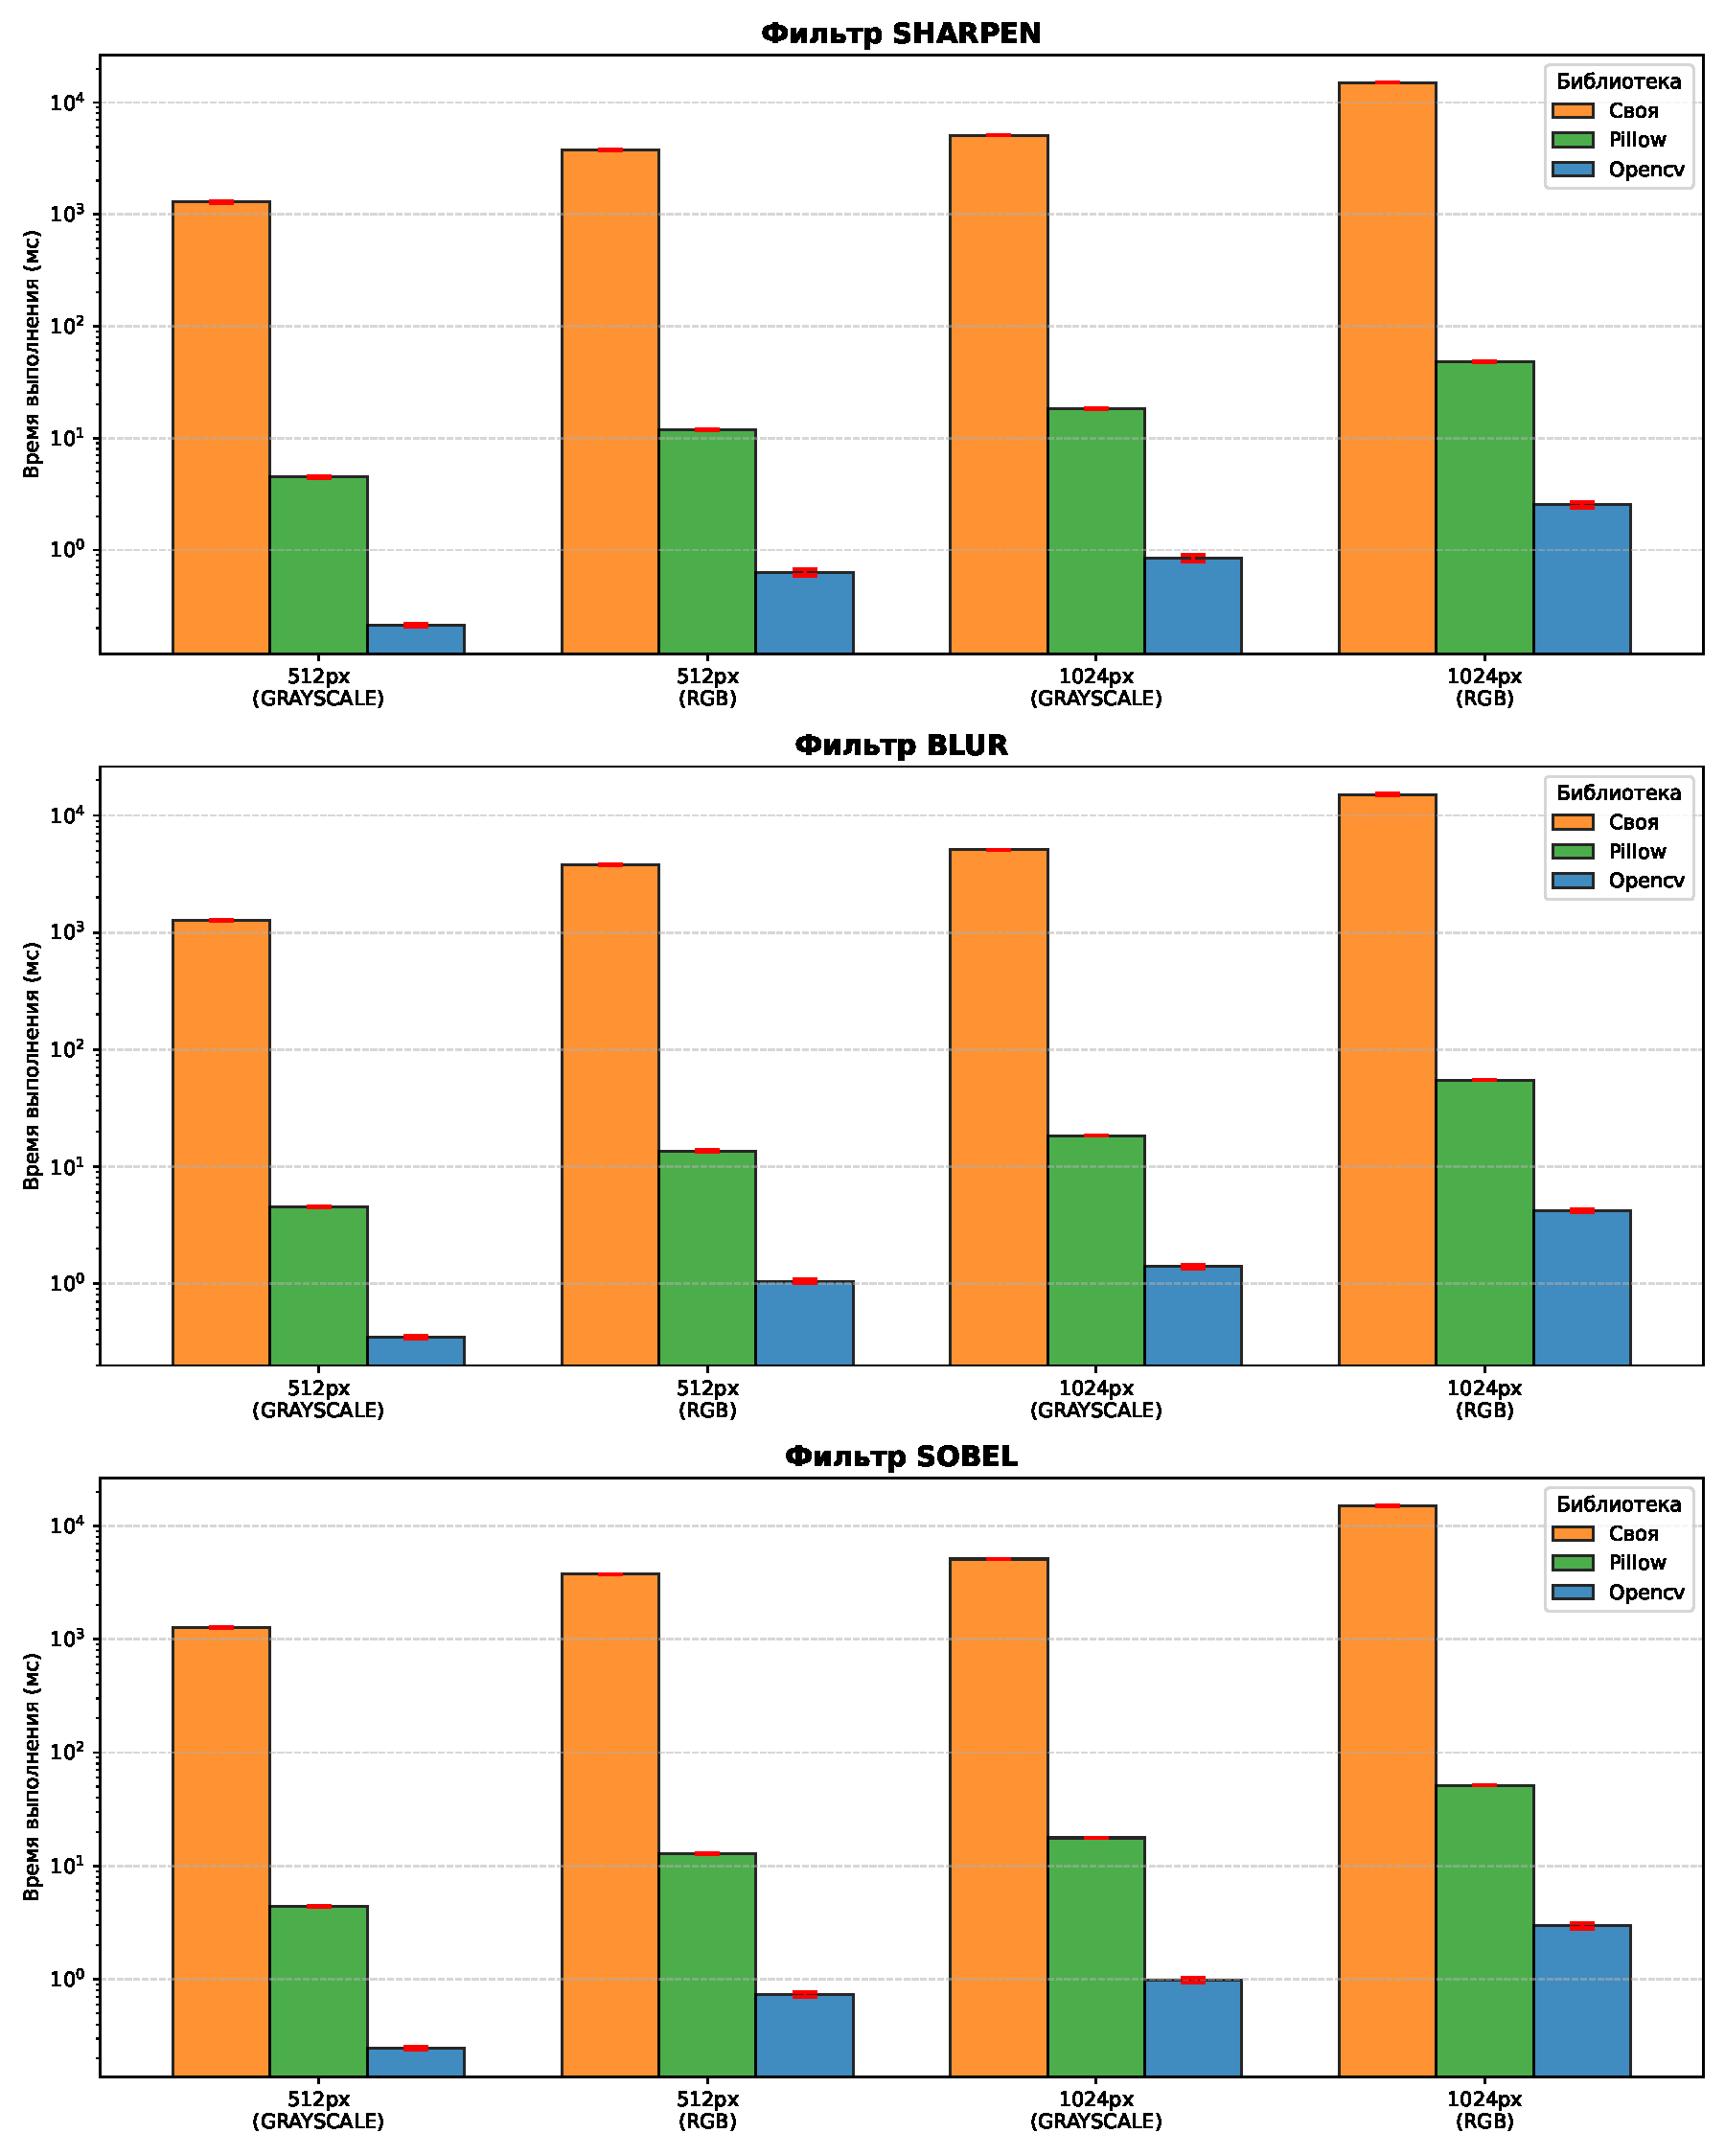
\includegraphics[width=0.5\textwidth]{benchmark.pdf}
    \caption{Сравнение производительности различных реализаций свёртки}
    \label{fig:benchmark}
\end{figure}

Результаты представлены на рисунке~\ref{fig:benchmark}.

Проведённые эксперименты позволяют сделать несколько выводов.
Во-первых, собственная реализация существенно уступает по скорости библиотечным решениям. В среднем она оказывается в несколько тысяч раз медленнее OpenCV и в несколько сотен раз медленнее Pillow.
Во-вторых, увеличение размера изображения приводит к росту времени выполнения для всех реализаций. При переходе от размера $512 \times 512$ к размеру $1024 \times 1024$ количество пикселей возрастает в четыре раза, что приводит к соответствующему увеличению времени обработки.
В-третьих, обработка RGB-изображений требует больше времени по сравнению с полутоновыми изображениями. Это связано с необходимостью выполнять свёртку отдельно для каждого цветового канала.
Наиболее высокую производительность показала библиотека OpenCV, что объясняется использованием низкоуровневых оптимизаций и реализацией основных алгоритмов на языке C++.

\section{Заключение}

В ходе выполнения учебной практики была разработана собственная реализация операции двумерной свёртки изображений на языке Python.

В результате работы:
\begin{itemize}
    \item реализована поддержка полутоновых и RGB-изображений;
    \item реализованы различные режимы обработки границ изображения;
    \item реализован набор свёрточных фильтров;
    \item разработаны интеграционные для проверки корректности работы;
    \item проведено исследование производительности;
    \item выполнено сравнение с библиотеками OpenCV и Pillow.
\end{itemize}

Полученные результаты показали корректность реализованного алгоритма и подтвердили преимущество специализированных библиотек по скорости выполнения. При этом разработанная реализация позволяет наглядно изучить принцип работы свёртки изображений и особенности её применения на практике.

Репозиторий проекта: \url{https://github.com/MariiaByvalkina/image-convolution-practice}

\end{document}
